\documentclass[10pt]{paper}

\usepackage[tmargin=1.5in, lmargin=0.55in, rmargin=0.55in, bmargin=1.0in]{geometry}


\usepackage{typewriter}
\usepackage{graphicx}
\usepackage{multirow}

\title{ On the relationship between rabbit-skinners and poppy-chewers }


\author{Pr Fancy stone}

\begin{document}

\section*{Abstract}
This paper re-evaluate the history of Rabbithole and its two main populations (the ``Poppy-chewers'' and the ``Rabbit-skinner'') using all the published set of dates spanning from 7400BP to 6500BP, from almost 40 settlements of central and Western Rabitthole, including all the most recent publication by Stone et al. 2022. To explore the history of the region and the relationship between its original habitants, we developed a specific quantitative method called ``Test of Balanced Equilibrium'' (TBE), to demonstrate that Rabbit-Skinner and Poppy-Chewer, though radically different in term of subsistence strategies, were having very intense and peaceful interactions.

\section{Introduction}
Understanding the relationships between Hunter Gatherer and Farmer has been  
\section{Method}

\pagebreak


To show that we are obviously right, we designed a brand new and powerful mathematical tool that we called: ``Test for Balanced Equilibrium''. This tool relies on very clever use of mathematics and has, to our knowledge, never been used in any scientific context so far. It allows to highlight relationship between geographical areas and quantitatively show when they are basically in a peaceful equilibrium.

\begin{figure}[hbp]

    \centering
    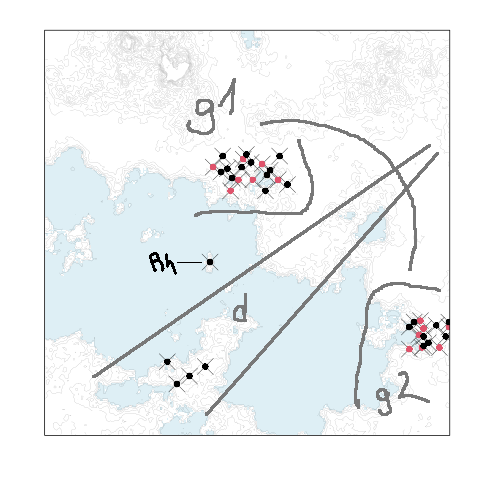
\includegraphics[width=.65\textwidth]{all_gpe.png}
    \caption{Map of rabbit with all published settlement}
    \label{fig:newage}
\end{figure}


To do that we group the settlement in 4 groups: the two firsts being the group from the old ages, the second the groups from the new ages 



\begin{equation}
    TEB= \left( N_i - N_j\right)
\end{equation}

\pagebreak

\section{Results}

\begin{figure}
    \centering
    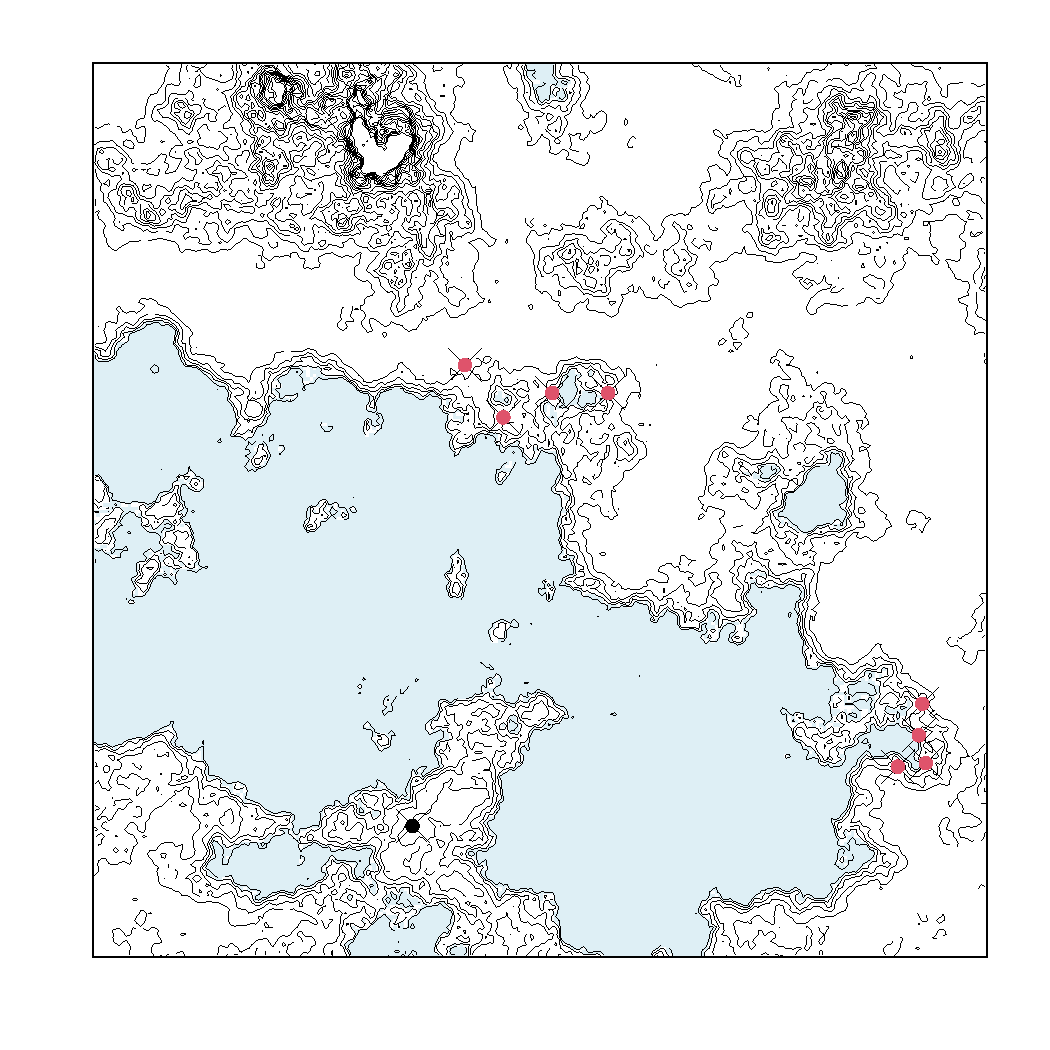
\includegraphics[width=.65\textwidth]{oldages}
    \caption{Map of rabbit hole during the Old age (~7200 - 7000 BP)  }
    \label{fig:allage}
\end{figure}

\begin{figure}
    \centering
    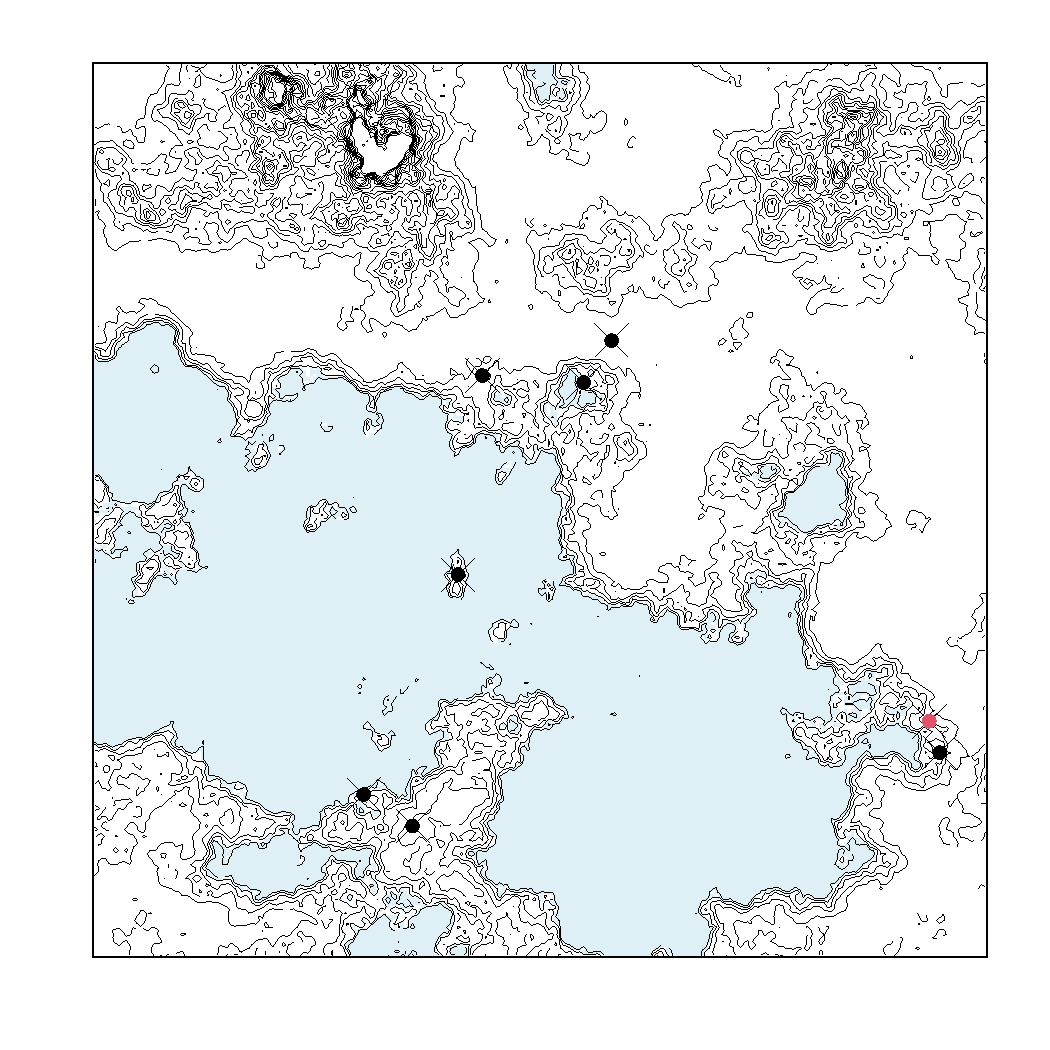
\includegraphics[width=.65\textwidth]{newages}
    \caption{Map of Rabbit hole after Farmer extension  (~7000 - 6800 BP)  }
    \label{fig:oldage}
\end{figure}
\begin{figure}
    \centering
    \makebox[\textwidth][c]{
    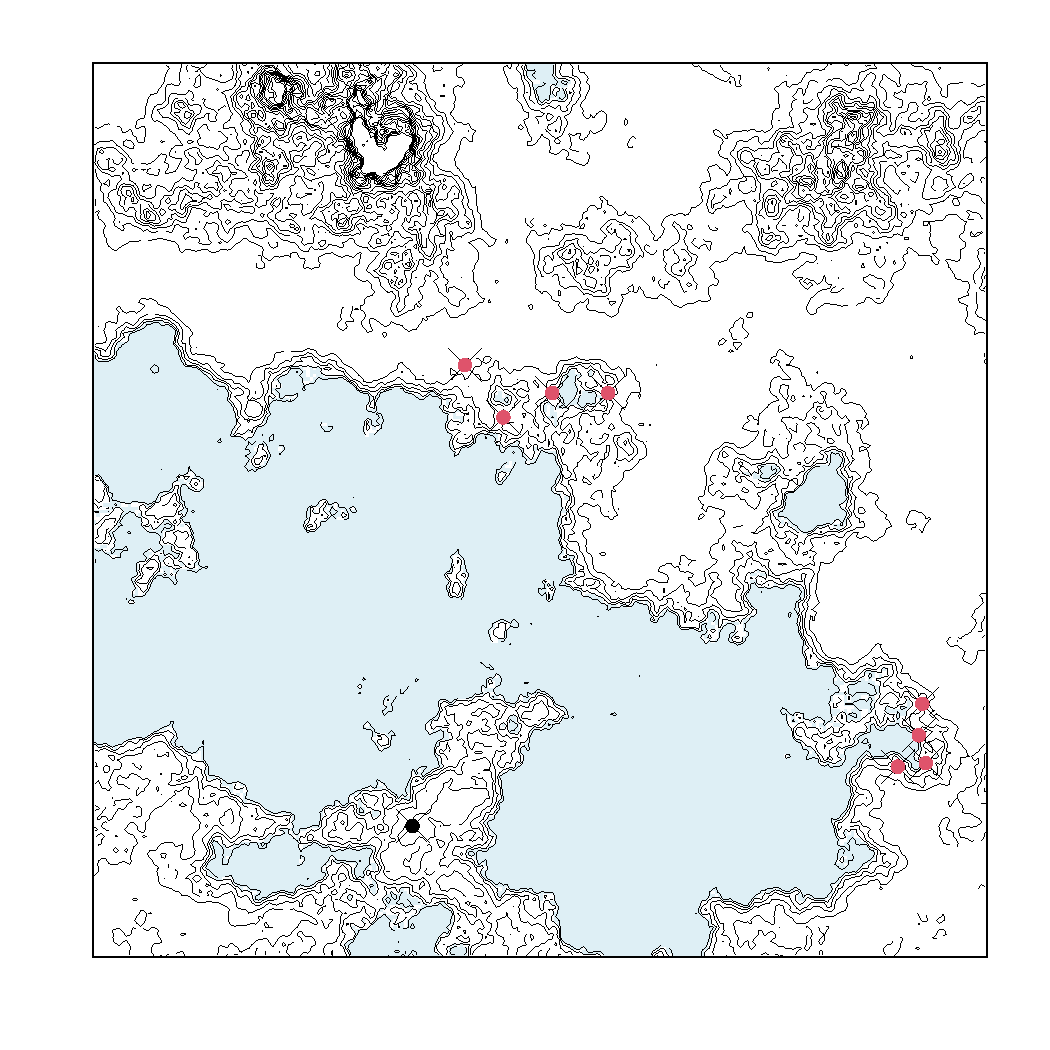
\includegraphics[width=.75\textwidth]{oldages}
    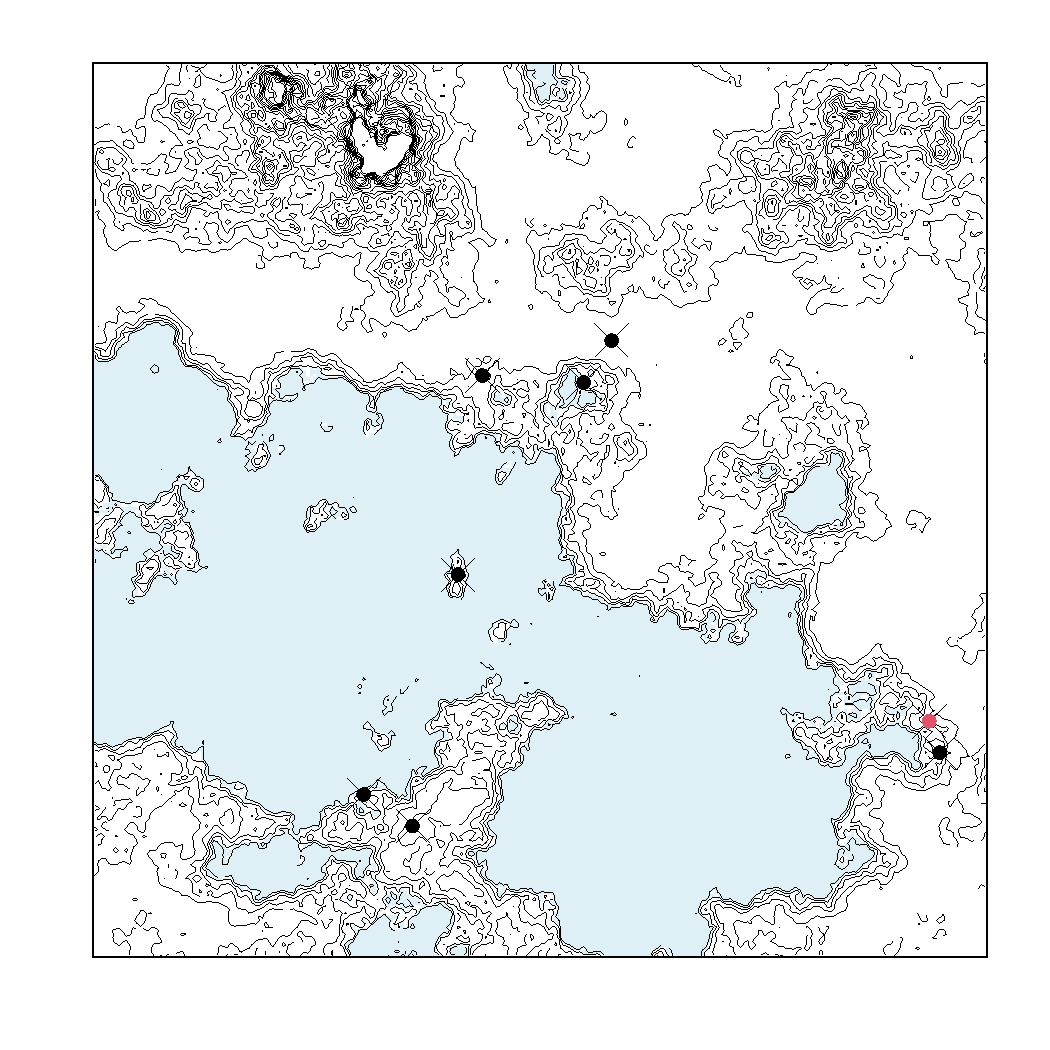
\includegraphics[width=.75\textwidth]{newages}
}
    \caption{Map of rabbit hole during the Old age (~7200 - 7000 BP) on the left, after Farmer extension  (~7000 - 6800 BP) on the right }
    \label{fig:twomaps}
\end{figure}
\end{document}

